 % Referencia: MDA. Engeenering emergency (dorman's)

% ---------------------------------------------------------------------------- %
\chapter{Fundamentos}
\label{cap:fundamentos}
% ---------------------------------------------------------------------------- %

Para se criar e treinar uma inteligência artificial, diversos arcabouçous são necessários. Por um lado, existe a parte teórica e matemática na qual a inteligência se baseia para aprender. Por outro, do lado computacional, existem as bibliotecas que auxiliam no desenvolvimento, efetuando as contas necessárias e, neste trabalho em particular, emulando o jogo que serve de ambiente para o aprendizado.
Este capítulo tem o intuito de familiarizar o leitor com a teoria e as ferramentas utilizadas no treinamento da inteligência artificial deste trabalho.

% ---------------------------------------------------------------------------- %
% https://en.wikipedia.org/wiki/Asteroids_(video_game)
% https://en.wikipedia.org/wiki/Golden_age_of_arcade_video_games
% https://www.arcade-museum.com/game_detail.php?game_id=6939
% https://www.ranker.com/list/the-most-popular-golden-age-arcade-games/video-games-lists
\section{Asteroids}
\label{sec:asteroids}

Asteroids é um jogo de fliperama do gênero shooter (jogo eletrônico de tiro) lançado em novembro de 1979 pela então desenvolvedora de jogos eletrônicos Atari.
O jogador controla uma nave espacial que se encontra em um campo de asteróides e precisa atirar para destruir todos eles ao mesmo tempo que evita colisões. O jogo se torna mais difícil conforme o número de asteróides na tela aumenta.

Diversas versões deste jogo foram criadas ao longo dos anos. Além das diferenças gráficas, as mudanças incluem naves espaciais inimigas que atiram contra o jogador, e tamanhos e formatos diferentes que os asteróides podem ter.

Para este trabalho, Asteroids foi emulado utilizando a plataforma Gym-Retro da companhia de pesquisas de inteligência artificial OpenAI. Todas as informações sobre o jogo apresentadas a seguir referem-se a tal versão.
Para o aprendizado da inteligência artificial, não há naves inimigas e os asteróides podem assumir três tamanhos e três formatos distintos. Os tamanhos são grande (inicial), médio e pequeno, enquanto os formatos são consideravelmente parecidos.
Há cinco comandos disponíveis: mover-se para frente, girar a nave no sentido horário, girar a nave no sentido anti-horário, atirar para frente, e entrar no hiper espaço. Mover-se para frente e girar no sentido horário ou anti-horário são as principais formas de movimento disponíveis ao jogador, e atirar serve para destruir os asteróides. Mover-se no hiper espaço consiste em fazer a nave desaparecer e, depois de alguns instantes, reaparecer em um local aleatório da tela. Há o risco de reaparecer em cima de um asteróide e, com isso, ter a nave destruída.
A nave possui aceleração e desaceleração, ou seja, inércia, de forma que, mesmo que o jogador deixe de pressionar o botão de mover-se para frente, a nave continuará em movimento por um curto período de tempo antes de parar por completo. Isso gera um grau a mais de complexidade, pois faz com que manobras de esquiva e curvas sejam mais difíceis de serem devidamente executadas.
Asteroids é considerado um dos primeiros grandes sucessos da era de ouro dos jogos de fliperama, que é a época em que os jogos eletrônicos se estabeleceram como uma força dominante na cultura popular.

% ---------------------------------------------------------------------------- %
% https://github.com/openai/retro
% https://blog.openai.com/gym-retro/
% https://openai.com/
% https://gym.openai.com/
\section{Gym-Retro}
\label{sec:gymretro}

Gym-Retro é uma plataforma para pesquisa de aprendizado por reforços e generalização em jogos desenvolvida e mantida pela empresa de pesquisas em inteligência artificial OpenAI. O lançamento mais recente inclui jogos do Sega Genesis, Sega Master System, Nintendo Entertainment System (NES), Super Nintendo Entertainment System (SNES) e Nintendo Game Boy, além de suporte preliminar para Sega Game Gear, Nintendo Game Boy Color, Nintendo Game Boy Advance e NEC TurboGrafx. Em qualquer um desses consoles, a ROM (Read Only Memory) do jogo é necessária.
Apesar de não ter sido utilizada neste trabalho, a plataforma disponibiliza uma ferramente que permite criar save states (salvar um estado a partir do qual é possível continuar o jogo), encontrar locais da memória, criar cenarios para o agente resolver, gravar e passar arquivos de vídeo, dentre outras funcionalidades.
Gym-Retro baseia-se na ferramenta Gym, desenvolvida e mantida pela OpenAI, que também tem como objetivo pesquisas em aprendizado por reforço, mas não apenas para jogos.

\begin{displayquote}
  \textit{Game Design é o ato de decidir como um jogo deve ser.}\footnote{Tradução livre feita pelo autor}
\end{displayquote}

\begin{displayquote}
  \textit{Os documentos gravam decisões feitas e concordadas oralmente [entre os integrantes do grupo]; (...) mais importante que isso, eles transformam ideias vagas em planos explícitos.}\footnote{Tradução livre feita pelo autor}
\end{displayquote}

\begin{lstlisting}
  while (true)
  {
    processInput();
    update();
    render();
  }
\end{lstlisting}

% ---------------------------------------------------------------------------- %
\section{Técnicas}
\label{sec:tecnicas}

Apesar de grande parte do desenvolvimento de \textit{PsyChO: The Ball} ter sido feita apenas por uma pessoa, foi muito benéfica a utilização de sistemas de versionamento que ajudam tanto na centralização de todo o código do jogo, facilitando na transição entre ambientes de trabalho, quanto na possibilidade de guardar versões antigas e resgatar códigos passados quando necessário. Durante todo o desenvolvimento de \textit{PsyChO: The Ball} foi utilizado um sistema de controle de versão para código e nele se encontram todas as versões de lançamento do jogo.

Uma boa prática na produção de um jogo, seja esse comercial ou um projeto pessoal, é a de lançamentos, ou \textit{releases}, constantes. O propósito disto é ter, periodicamente, \textit{releases} de versões estáveis e jogáveis do jogo, de forma que outras pessoas possam jogar e dar \textit{feedback} frequente, assim ajudando no encaminhamento do projeto. Essa técnica é muito comum em metodologias ágeis de desenvolvimento de software e essa linha de pensamento foi o que guiou todo o desenvolvimento de \textit{PsyChO: The Ball}.

Inicialmente foi utilizado o sistema \textit{Kanban}, uma abordagem moderna de conceitos ágeis muito comum em empresas ou grupos de desenvolvimento de software. Kleber Bernardo, especialista em métodos ágeis, descreve bem a metodologia em um artigo no site Cultura Ágil \cite{kleberkanban}:

\begin{displayquote}
  \textit{O Kanban lhe ajuda a assimilar e controlar o progresso de suas tarefas de forma visual. É, normalmente, utilizado um quadro branco com alguns pequenos papéis (Post-it) colados, esses papéis representam as suas tarefas, ao termino de cada tarefa o papel é puxado para a etapa seguinte até que a mesma seja finalizada. Ao olhar para um quadro Kanban é fácil enxergar como o trabalho seu e de sua equipe fluem, permitindo não só comunicar o status, mas também dar e receber feedbacks.}
\end{displayquote}

\begin{figure}[h!]
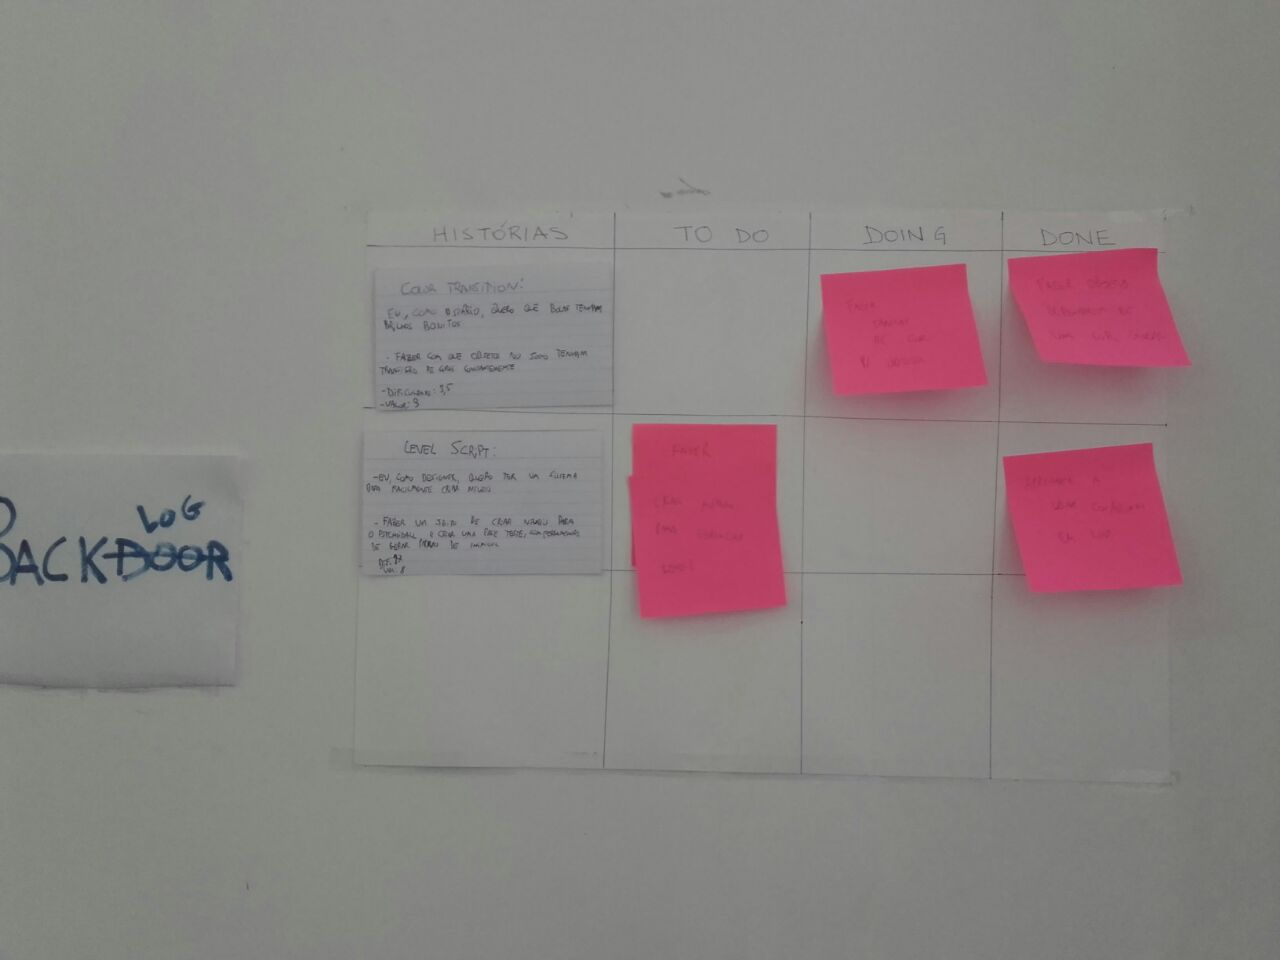
\includegraphics[scale=.3]{kanban}
\centering
\caption{Kanban utilizado durante o desenvolvimento de \textit{PsyChO: The Ball}}
\end{figure}

Entretanto, após alguns meses utilizando essa técnica, o tempo gasto em sua manutenção acabou se tornando mais trabalhoso do que produtivo para o projeto e seu uso foi decaindo. Desta forma o \textit{Kanban} foi substituido por várias pequenas técnicas ágeis, como lançamentos frequentes do jogo, \textit{sprints} (onde era determinado um prazo de uma ou duas semanas para terminar funcionalidades no jogo) e constantes re-avaliações com consulta de \textit{feedback}.

Por último, uma técnica muito presente no desenvolvimento do jogo foi a utilização de documentação para marcar mudanças e melhorias no projeto. Os dois documento mais importantes são o \textit{DEVLOG}\footnote{https://github.com/uspgamedev/Project-Telos/blob/dev/docs/DEVLOG.md} e \textit{CHANGELOG}\footnote{https://github.com/uspgamedev/Project-Telos/blob/dev/docs/CHANGELOG.md}. O \textit{DEVLOG} foi um necessário para mostrar o progresso e tempo gasto no projeto, enquanto este fazia parte da disciplina \textit{MAC0214 Atividade Curricular em Cultura e Extensão}. Nele existem várias entradas detalhando atividades feitas no jogo durante o desenvolvimento. O \textit{CHANGELOG} por outro lado serve para marcar lançamentos do jogo, descrevendo \textit{features} novos adicionados em cada \textit{sprint} feito. Ambos documentos foram de grande utilidade no início do desenvolvimento de \textit{PsyChO: The Ball}, pois exibem concretamente o fluxo de progresso na criação do jogo.

% ---------------------------------------------------------------------------- %
\section{Ferramentas}
\label{sec:ferramentas}

Uma das escolhas feitas para o desenvolvimento de \textit{PsyChO: The Ball} foi a utilização exclusiva de \textit{Software Livre}. Essa decisão se deu tanto pela liberdade que essas ferramentas permitem em sua utilização, quanto pelo objetivo de incentivar mais o uso desse tipo de software, mostrando que é tão eficiente quanto o uso de software proprietário. Assim, como critério de escolha para cada área de desenvolvimento do jogo, foi determinado algum software livre que tenha uma comunidade ativa (para a solução de problemas e disponibilidade de bibliotecas), constante atualização de suas funcionalidades, versões estáveis e uma recomendação de seu uso no desenvolvimento de jogos.

O arcabouço utilizado no desenvolvimento de \textit{PsyChO: The Ball} foi a \textit{Love2d} ou \textit{LÖVE}\footnote{https://love2d.org/}, uma \textit{framework} gratuita que utiliza a linguagem \textit{Lua}\footnote{https://www.lua.org/portugues.html}.

Como sistema de controle de versão foi utilizado \textit{Git}\footnote{https://git-scm.com/} através da plataforma de uso grátis \textit{Github}\footnote{https://github.com/}.

Para a produção de música foi utilizado \textit{LMMS}\footnote{https://lmms.io/}, um software livre gratuito para manipulação e criação de sons.

Por último, para manipulação de imagens, foi utilizada a ferramenta \textit{Gimp}\footnote{https://www.gimp.org/}.

\begin{figure}[h!]

\includegraphics[scale=.5]{icons}
\centering
\caption{Da esquerda pra direita, ícones de \textit{LÖVE}, \textit{Lua}, \textit{Git}, \textit{Github}, \textit{LMMS} e \textit{Gimp}}
\end{figure}

Dentre essas ferramentas, vale ressaltar um ponto muito interessante do arcabouço \textit{LÖVE}: seu \textit{gameloop} tem o diferencial de deslocar todas as verificações de \textit{input} do usuário como \textit{callbacks assíncronos}. Estes são funções que a própria \textit{framework} vai chamar quando ocorrer algum \textit{input} do usuário, como quando ele pressionar um botão do teclado ou mover o mouse. Através de subrotinas, o arcabouço está constantemente aguardando sinais que ativem essas funções e assim o desenvolvedor não precisa se preocupar em lidar com otimização ou código confuso na hora de esperar e tratar comandos dados pelo usuário. Isso foi uma grande vantagem que determinou a escolha dessa ferramenta na produção de \textit{PsyChO: The Ball}.

% ---------------------------------------------------------------------------- %
